\renewcommand*{\arraystretch}{1.1}

\noindent\begin{tabularx}{17cm}{|p{1.95cm}|X|}
	\hline
	workload    & Interactive / update \\ \hline
%
	query       & 6 \\ \hline
%
	title       & Add Post \\ \hline
%
    pattern     & \hfill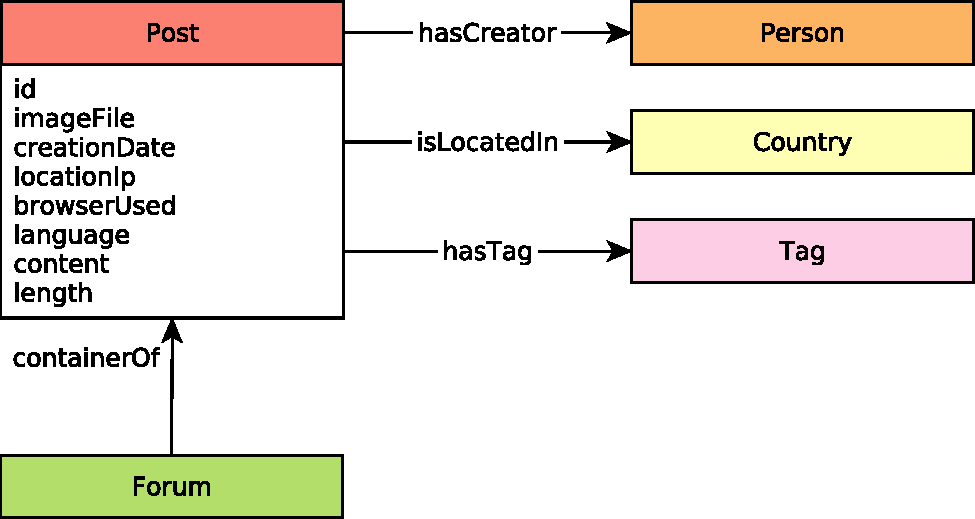
\includegraphics[scale=\patternscale,margin=0cm .2cm]{patterns/interactive-update-06}\hfill\vadjust{} \\ \hline
%
	description & Add a Post to the social network.
 \\ \hline
%
	
%
	parameters  &
	\vspace{1.1ex}{\begin{tabularx}{14.2cm}{|c|M|m{2cm}|Y|} \hline
	\cellcolor{parameter} \color{white} $\mathsf{1}$ & \varname{Post.id} & \cellcolor{gray!20} \vartype{ID} &  \\ \hline
	\cellcolor{parameter} \color{white} $\mathsf{2}$ & \varname{Post.imageFile} & \cellcolor{gray!20} \vartype{String} &  \\ \hline
	\cellcolor{parameter} \color{white} $\mathsf{3}$ & \varname{Post.creationDate} & \cellcolor{gray!20} \vartype{DateTime} &  \\ \hline
	\cellcolor{parameter} \color{white} $\mathsf{4}$ & \varname{Post.locationIp} & \cellcolor{gray!20} \vartype{String} &  \\ \hline
	\cellcolor{parameter} \color{white} $\mathsf{5}$ & \varname{Post.browserUsed} & \cellcolor{gray!20} \vartype{String} &  \\ \hline
	\cellcolor{parameter} \color{white} $\mathsf{6}$ & \varname{Post.language} & \cellcolor{gray!20} \vartype{String} &  \\ \hline
	\cellcolor{parameter} \color{white} $\mathsf{7}$ & \varname{Post.content} & \cellcolor{gray!20} \vartype{Text} &  \\ \hline
	\cellcolor{parameter} \color{white} $\mathsf{8}$ & \varname{Post.length} & \cellcolor{gray!20} \vartype{32-bit Integer} &  \\ \hline
	\cellcolor{parameter} \color{white} $\mathsf{9}$ & \varname{Post-hasCreator->Person.id} & \cellcolor{gray!20} \vartype{ID} &  \\ \hline
	\cellcolor{parameter} \color{white} $\mathsf{10}$ & \varname{Post<-containerOf-Forum.id} & \cellcolor{gray!20} \vartype{ID} &  \\ \hline
	\cellcolor{parameter} \color{white} $\mathsf{11}$ & \varname{Post-isLocatedIn->Country.id} & \cellcolor{gray!20} \vartype{ID} &  \\ \hline
	\cellcolor{parameter} \color{white} $\mathsf{12}$ & \varname{\{Post-hasTag->Tag.id\}} & \cellcolor{gray!20} \vartype{\{ID\}} &  \\ \hline
	\end{tabularx}}\vspace{1.1ex} \\ \hline
%
	
%
	%
	%
	%
\end{tabularx}
\vspace{2ex}